\documentclass[12pt]{scrartcl}
\usepackage[utf8]{inputenc}
\usepackage[ngerman]{babel}

\usepackage{fancyhdr}
\usepackage{graphicx}
\usepackage{enumerate}
\fancyhf{}
\pagestyle{fancy}

\pagestyle{fancy}

\fancyhead[R]{Prof. Dr. Gerit Wagner}
\fancyhead[L]{Git exercise}
%\renewcommand{\headrulewidth}{0.5pt}
%hallowelt
\begin{document}
~
\medskip
    \begin{center}
      \textbf{\large{Exercise on Git}}\\
    \end{center}

\vspace{0.5cm}
\noindent
You work on a research paper with two fellow students. To collaborate effectively, the team has decided to use Git and Markdown, as well as Pandoc to generate outputs such as pdf, tex, html, or docx. As part of the project, complete the following steps and enter the required commands.

\vspace{0.5cm}

\noindent
You have created a README.md file in an empty directory. Initialize a git repository, and create a commit containing this file:

\vspace{0.5cm}

\hrulefill

\vspace{0.5cm}

\hrulefill

\vspace{0.5cm}

\hrulefill

\vspace{0.5cm}
\noindent
Briefly summarize the state of the three git sections afterwards:
\vspace{0.5cm}

\hrulefill

\vspace{0.5cm}

\hrulefill

\vspace{0.5cm}

\hrulefill

\vspace{0.5cm}
\noindent
You work on the REAMDE.md, CONTRIBUTING.md and paper.md files. All changes should be part of the next commit (do not yet create the commit):

\vspace{0.5cm}

\hrulefill

\vspace{0.5cm}
\noindent
You decide that the paper.md changes should be part of a separate commit. Use the appropriate operations to accomplish this:
\vspace{0.5cm}

\hrulefill

\vspace{0.5cm}

\hrulefill

\vspace{0.5cm}

\hrulefill

\vspace{0.5cm}

\hrulefill

\vspace{0.5cm}
\newpage
\noindent
At some point, you notice that the paper.md file is in two sections (to be committed and not staged for commit), as indicated by git status:

\begin{verbatim}
On branch main
Your branch is up to date with 'origin/main'.

Changes to be committed:
(use "git restore --staged <file>..." to unstage)
modified:   paper.md

Changes not staged for commit:
(use "git add <file>..." to update what will be committed)
(use "git restore <file>..." to discard changes in working directory)
modified:   paper.md
\end{verbatim}
\noindent
Explain what this means and whether this is a valid state.

\vspace{0.5cm}

\hrulefill

\vspace{0.5cm}

\hrulefill

\vspace{0.5cm}

\noindent
The team plans to develop a section of the paper in a separate branch. This can be accomplished based on the following operations:

\vspace{0.5cm}

\hrulefill

\vspace{0.5cm}

\hrulefill

\vspace{0.5cm}

\hrulefill

\vspace{0.5cm}

\hrulefill

\vspace{0.5cm}

\noindent
The deadline for your work is in one week. To complete the project in time, sections one (introduction) and five (discussion) must be developed in parallel. Draw the Git graph with appropriate branch names:

\vspace{8cm}

\noindent
One day before the deadline, many commits were added to the main branch and the branches for sections one and five are behind. Before merging, these branches should be up-to-date with the recent changes in main:

\vspace{0.5cm}

\hrulefill

\vspace{0.5cm}

\hrulefill

\vspace{0.5cm}

\noindent
Your colleague Anna has completed the introduction all by herself and updated the branch for section one by running

\vspace{0.3cm}

git rebase main \&\& git push -f.

\vspace{0.3cm}

\noindent
Explain whether this is a suitable approach for the other branch, which contains work by Nicole, Tim, and Sandy.
\vspace{0.5cm}

\hrulefill

\vspace{0.5cm}

\hrulefill

\vspace{0.5cm}

\hrulefill

\vspace{0.5cm}

\noindent
The state of the local and remote discussion branches is the following:

\begin{center}
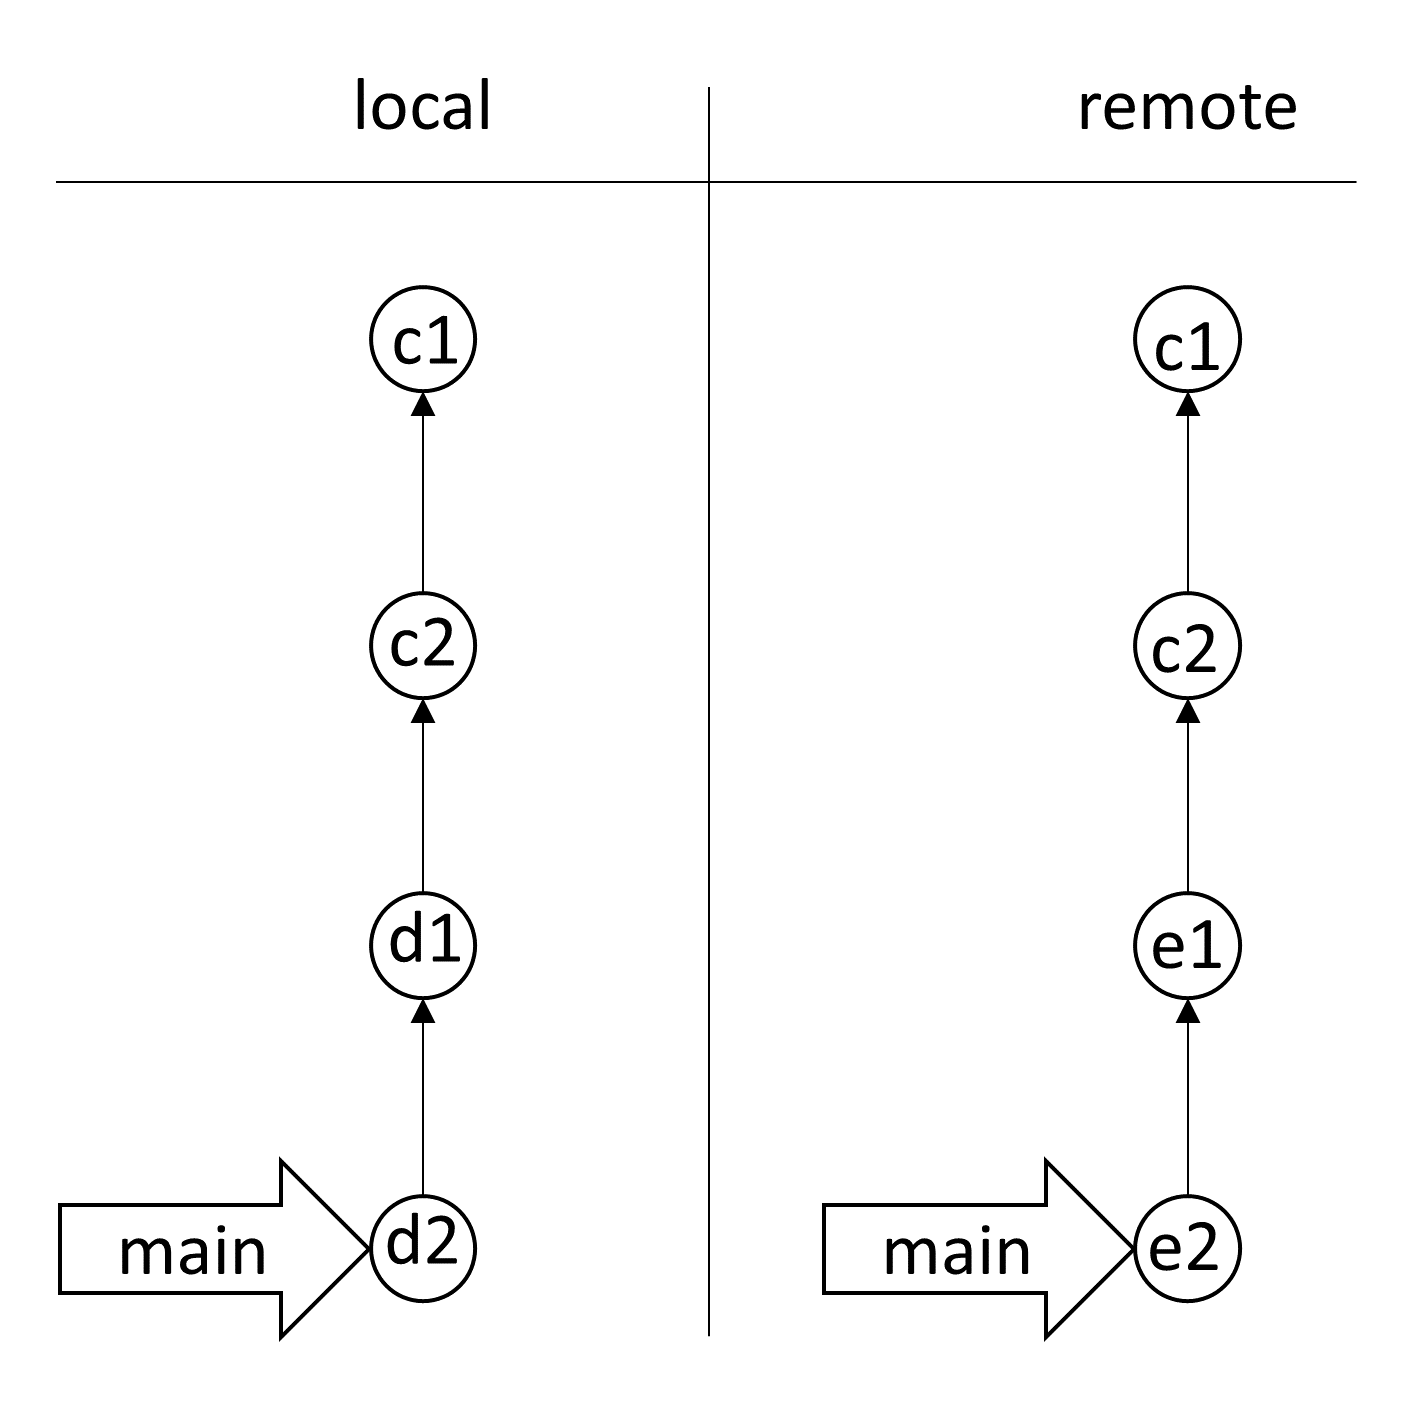
\includegraphics[scale=0.5]{git-graph_1.png}
\end{center}

\noindent
Running git pull gives you an error, which states that you "Need to specify how to reconcile divergent branches". Identify the diverging commits and draw the git graph after completing git pull --rebase:

\vspace{10cm}
\newpage
\noindent
In another project, gitk shows the following overview of commits and branches (most recent on top). HEAD currently points to main.

\vspace{0.5cm}

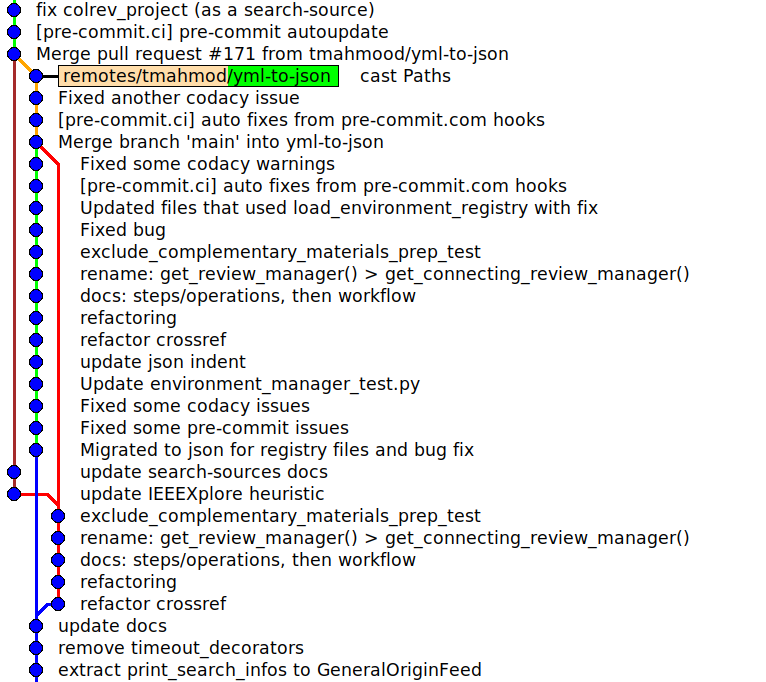
\includegraphics[scale=0.5]{gitk.png}

\vspace{0.5cm}

\noindent
Provide the git commands leading to this graph (similar to learngitbranching). You can use "3x commit" to create three commits in a row. 

% TODO : take an example from the DPKW paper (it may contain commits resembling a research paper)

\end{document}
